\documentclass{article}

%usepackages
\usepackage[utf8]{inputenc}
\usepackage{graphicx}
\usepackage[normalem]{ulem}
\usepackage{enumitem}
\usepackage{amsmath}
\usepackage{cancel}
\usepackage{amssymb}
\usepackage{hyperref}
\usepackage{tikz}
\usepackage[english]{babel}
\usepackage[letterpaper, portrait, margin=1.2in]{geometry}
%\usepackage{fancyhdr}

%new commands
\newcommand{\R}{\mathbb{R}}
\newcommand{\N}{\mathbb{N}}
\newcommand{\Q}{\mathbb{Q}}
\newcommand{\Z}{\mathbb{Z}}
\newcommand{\C}{\mathbb{C}}
\newcommand{\inv}{^{-1}}
\newcommand{\img}{\textmd{Im}\:}
\newcommand{\cok}{\textmd{coker}}
\newcommand{\conv}{\textmd{conv}}
\newcommand{\vertices}{\textmd{vert}}
\newcommand{\st}{\textmd{ s.t. }}
\newcommand{\fracfield}{\textmd{frac}\:}

%new theorem environments
\newtheorem{definition}{Definition}[section]
\newtheorem{lemma}{Lemma}[section]
\newtheorem{example}{Example}[section]
%title
\title{Summary}
\author{Luca Bracone}
%TODO: THIS IS STILL VERY BAREBONES. ADD TEXT BEFORE EVERY SUBSECTION, EXPLAINATION AFTER NN DEFINITION REFERNCING IMAGE. ADD ABSTRACT. THE IMAGE IS IN SPANISH FIND ENGLISH ONE.
\begin{document}
	\maketitle
	\section{Basic Machine Learning}
	\subsection{Neural Networks}
	\begin{definition}[Perceptron]
		A \uline{Perceptron} is a function $ p:\R^n \to \R $ given by 
		\[ p(x_1, \dots , x_n) = g \left( w_0 + \sum_{i=1}^{n} w_i x_i \right)  \]
		Where $ w_1, \dots, w_n \in \R $ are called the \uline{weights} of $p$, $w_0$ is called the \uline{bias}, and $g:\R \to \R $ is any non-linear function called the \uline{activation}.
		Most of the time \[ g(x)=\frac{e^x}{e^x+1} \] the sigmoid function.
	\end{definition}
%	\begin{minipage}{0.3\textwidth}
%			\includegraphics[width=72px]{figure1.png}
%	\end{minipage}
%\begin{minipage}{0.7\textwidth}
	\begin{definition}[Artificial Neural Network]
		A (forward-feeding) \uline{Artificial Neural Network} (ANN) is a function $T: \R^n \to \R^m$ that can be decomposed as such \[ T= l_k \circ \dots \circ l_1  \] Where the $l_i : \R^{n_j} \to \R^{n_{j+1}}$ are called \uline{layers} and are essentially just vectors of perceptrons \[ l_i(\vec{x})=(p_{i,1}(\vec{x}),\dots,p_{i,n_j}(\vec{x})) \].
		In the context of neural networks perceptrons are also called nodes.
	\end{definition}
%\end{minipage}

\begin{definition}[Loss Function]
	For some ANN, $T$ and some input $ (x_1,...,x_n) $, we have a desired output $ (y_1,...,y_n) $ we would like $ T $ to match. Write $ (\hat{y}_1,...,\hat{y}_m) $ the output $T$ actually produced. The \uline{loss} (or sometimes, \uline{cost}) of $T$ for this input is a function that measures the "distance" between the produced and desired output. For most basic applications, 
	\[\mathcal{L}(W; x)= \sum_{i=1}^{m} ||y_i - \hat{y}_i||_2^2  \]
\end{definition}
\begin{definition}[Empirical Loss]
	For a set of inputs $X$, and $T$ a NN, the \uline{Empirical Loss} is 
	\[ J(W)=\frac{1}{|X|} \sum_{\vec{x}\in X} \mathcal{L}(W;x) \]
	the average loss over $X$.
\end{definition}

\subsection{Gradient Descent}
	Any neural network is defined by the weights of its perceptrons. Therefore, in order to have the neural network behave as desired (namely being as close as possible to the desired outputs) we need to find an efficient way to tweak the weights such that the empirical loss becomes as low as possible, when tested on some new inputs. Applying this algorithm repeatedly is called "training".
	\subsubsection{Gradient Descent}
		Essentially it involves taking a step in the "right" direction until we reach a stopping condition, most of the time it's when the steps we are taking are too short. In other words update the weights $W \gets W - \eta \nabla J$. Where $\eta$ is a constant that has to be well chosen. If too small, gradient descent stops when it meets the slightest uphill, and thus misses a better minimum which might be close by. If too big, gradient descent can only take giant steps and diverges to infinity.
	\subsubsection{Gradient Backpropagation}
		In practice, calculating the derivative to some particular weight is quite simple, consider the following neural net: \\ \\
		\begin{minipage}{0.55\linewidth}

		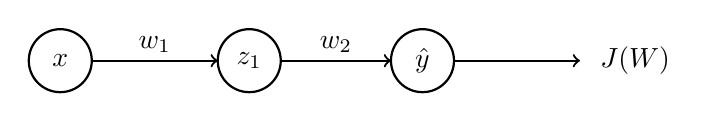
\begin{tikzpicture}
		\draw[thick] (0,0) circle [radius=0.4];
		\node at (0,0) {$x$};
		\draw[->, thick] (0.4,0) -- (2,0);
		\node at (1.2,0.2) {$w_1$};
		\draw[thick] (2.4,0) circle [radius=0.4];
		\node at (2.4,0) {$z_1$};
		\draw[->, thick] (2.8,0) -- (4.2,0);
		\node at (3.5,0.2) {$ w_2 $};
		\draw[thick] (4.6,0) circle [radius=0.4];
		\node at (4.6,0) {$ \hat{y} $};
		\draw[->,thick] (5,0)--(6.6,0);
		\node at (7.3,0) {$ J(W) $};
		\end{tikzpicture}
		\end{minipage}
	\begin{minipage}{0.45\linewidth}
		It's just an application of the chain rule:
		\begin{align*}
		\frac{\partial J}{\partial w_2} &=\frac{\partial J}{\partial \hat{y}} \frac{\partial \hat{y}}{\partial w_2} \\
		\frac{\partial J}{\partial w_1} &= \frac{\partial J}{\partial \hat{y}}\frac{\partial \hat{y}}{\partial z_1}\frac{\partial z_1}{\partial w_1}
		\end{align*}
	\end{minipage}
	\subsubsection{Data Batching}
	Since calculating $\nabla J$ is computationally intensive, consider taking a random subset of your data, and applying gradient descent to it instead. the convergence is going to be more erratic, depending on the size of the subset chosen, but the time gained makes it worth.
	\subsection{Overfitting}
	When training our neural network, it might happen that it essentially "learns the dataset by heart" making it unable to properly tackle on never seen before data points. There are a few methods to avoid such a problem:
		\begin{figure}[ht!]
		\centering
		\includegraphics{overfitting.png}
		\caption[image of overfitting]{A parabola+noise is being misunderstood as a complicated winding line \protect \footnotemark}
		\end{figure}
		\footnotetext{Courtesy of wikimedia foundation \href{https://commons.wikimedia.org/wiki/File:Overfitting.svg}{https://commons.wikimedia.org/wiki/File:Overfitting.svg}}
	\subsubsection{Dropout}
	This technique involves randomly setting some nodes to zero during training. This makes the network not rely too much on some path.
	\subsubsection{Early Stopping}
	After each application of gradient descent, test the network. If it performs worse than it did previously, stop the training process.	
	
	\section{Simplicial Complexes}
	\begin{definition}[convex hull]
	let $ u_0,...,u_k \in \R^n $ their convex hull is
	 \[ \conv \{u_0,...,u_k\} = \left\{ x= \sum_{i=0}^{n} \lambda_i u_i \ \st    \sum_{i=0}^{n} \lambda_i = 1; \ \lambda_i > 0 \ \forall i \right\} \qquad (\star) \]
	\end{definition}
	\begin{definition}[affinitely independent, $k$-simplex]
		$u_0,...,u_k \in \R^n$ are said to be affinitely independent if any point in their convex hull is written as in $(\star)$ uniquely.
		In that case instead of convex hull, we speak of $k$-simplex.
	\end{definition}
	\begin{definition} [face, coface]
		Let $ \{u_{i_0},...,u_{i_m} \} \subseteq \{u_0,...,u_k\} $ we say that $ \tau = \conv\{u_{i_1},...,u_{i_m}\} $ is a face of $ \sigma = \conv\{u_1,..,u_k\} $ which we write $ \tau < \sigma $. Equivalently $ \sigma $ is a co-face of $ \tau $.
	\end{definition}
	\begin{definition}[simplicial complex]
		A simplicial complex $K$ is a collection of simplices such that:
		\begin{enumerate}[label=(S\arabic*)]
			\item $ \forall \sigma \in K, \ \tau < \sigma \implies \tau \in K $. 
			\item $ \forall \sigma,\tau \in K, \ \sigma \cap \tau $ is either empty or a face.
		\end{enumerate}
	The dimension of $K$ is $ \dim K = \max_{\sigma \in K} \dim \sigma $ Where the dimension of a $k$-simplex is $k$.
	The Underlying space of $K$, $|K|$ is the topological space $ \bigcup_{\sigma \in K} \sigma $ with the subspace topology.
	\end{definition}
%todo:add examples of complexes
\begin{definition}[triangulation]
	Let $X$ be a topological space and $K$ a simplicial complex, if there exists a homeomorphism $ \phi : X \to |K| $ we say that $X$ is triangulable. In that case the couple $ (K,\phi) $ is called a triangulation of $X$
\end{definition}
	\begin{definition}[sub-complex]
		A subset $L \subseteq K$ is a subcomplex of K, if it is itself a complex. It is called full if it contains all vertices of $K$.
	\end{definition}
	\begin{example}[skeleton]
		The $j$-skeleton of complex $K$ is $K^{(j)}= \{ \sigma \in K \st \dim\sigma \leq j \} \subseteq K $. In particular the 0-skeleton is called $\vertices(K)$ the vertices of $K$
	\end{example}
	\begin{definition}[star and link]
		Let $K$ be a simplicial complex and pick $ \sigma \in K $. Its star, $ st\sigma = \{ \tau \in K \st \tau < \sigma \} $. unfortunately it's not a sub-complex of $K$ because it's not closed under taking faces. For that we define the closed star $ \overline{st}\sigma $ the smallest sub-complex that contains the star.
		%todo explain this better
		Similarly, the link of a simplex $ lk\sigma = \{ \tau \in \overline{st}\sigma \st \tau \cap \sigma = \emptyset \} $ the set of simplices in the closed star that don't touch $\sigma$
	\end{definition}
	\begin{definition}[simplicial maps, homeomorphisms]
		Let $K$, $L$ be two simplicial complexes and $ \phi: \vertices K \to \vertices L $ a map such that vertices of every simplex in $K$ gets mapped to a vertex of a simplex in $L$, in that case $\phi$ is called a vertex map.The map $f: |K| \to |L|$ defined by $ \sum_{i=0}^n \lambda_i u_i \mapsto \sum_{i=0}^n \lambda_i \phi(u_i) $ is called a simplicial map. If $ \phi $ is bijective and $ \phi\inv $ is also a vertex map, we speak instead of simplicial homeomorphism.
	\end{definition}

	\section{Simplicial Homology}
	\begin{definition}[p-chain]
		Let $K$ be a simplicial complex $ p $-chains are formal sums of $p$-simplices of $K$ over a field: \[ c = \sum_{i=1}^{n} a_i \sigma_i \] componentwise addition makes it into a commutative group $ (C_p, +) $. For the time being the field in question is $ \mathbb{F}_2 $.
	\end{definition}
\begin{definition}[boundary]
	the boundary of a $ p $-simplex is the sum of its $ (p-1) $-faces: \[ \partial_p c = \sum_{j=1}^n [\sigma_1, \dots , \cancel{\sigma_j} , \dots , \sigma_p] \]
\end{definition}

Turns out $ \partial_p : C_p \to C_{p-1} $ is a group homomorphism. for a simplicial complex $K$ we define its chain complex:
\[\mathcal{C}_K: \ \dots \longrightarrow C_p \stackrel{\partial_p}{\longrightarrow} C_{p-1} \stackrel{\partial_{p-1}}{\longrightarrow} \dots \stackrel{\partial_1}{\longrightarrow} C_0 \]

\begin{lemma}[Fundamental of Homology]
	For all $p$, $d \in C_{p+1}$, we have $ \partial_{p} \partial_{p+1} d = 0$
	%todo: add proof ??
\end{lemma}

Whenever we have an interesting homomorphism it is natural to want to know more about its kernel and image, in this case they have special names
\begin{definition}[$p$-boundaries and $p$-cycles]
	$p$-cycles are $ \ker\partial_{p} = \{ c \in C_p \st \partial c = 0 \} = Z_p $\\
	$p$-boundaries are $ \img\partial_{p+1} = \{ c \in C_p \st \exists d \in C_{p+1} , \ c=\partial d \} = B_p $
\end{definition}

Note that if $ c \in B_p $ then $ \partial c = \partial \partial d = 0 $ so, $ B_p \subseteq Z_p $. But in general $ Z_p \neq B_p $ in particular we are interested in the $p$-cycles that are not $p$-boundaries.
\begin{definition}[homology groups and Betti numbers]
	for a complex $K$ its $p$-th homology group is the quotient $H_p Z_p/B_p $.\\
	The $p$-th Betti number is $ \beta_p $ the number of generators of $H_p$.
\end{definition} 

%todo: write example

\begin{definition}[induced map]
	Consider two complexes $K$, $L$ and a simplicial map $ f: K \to L $. We have a way to transform $f$ into a map $ f_\sharp: C_p(K) \to C_p(L) $, in this way 
	\[ c = \sum_{i=1}^n a_i \sigma_i \ \mapsto \ \sum_{i=1}^{??} a_i \tau_i  \]
	Where $ \tau_i = f(\sigma_i) $ if it has dimension $p$ or $ \tau_i =0 $ otherwise. $f_\sharp$ is the induced map of $f$.
\end{definition}

%todo: more examples

\end{document}